\section{1174035 - Luthfi Muhammad Nabil}
Kecerdasan buatan merupakan kecerdasan yang dimasukkan ke sistem yang dapat diatur untuk kepentingan ilmiah. Kecerdasan buatan biasa disebut AI (Artificial Intelligence) yang didefinisikan sebagai kecerdasan ilmiah. AI memiliki kemampuan untuk menerjemahkan data dari luar, dan mempelajari data tersebut untuk dipelajari demi mencapai tujuan dan melakukan tugas tertentu sesuai hasil adaptasi berdasarkan data yang didapat. 

\subsection{Sejarah dan perkembangan Kecerdasan Buatan}
AI mulai berkembang sesuai dengan konsep yang dikemukakan pada awal abad 17, Rene Descartes menyebutkan bahwa tubuh hewan bukanlah apa-apa melainkan mesin-mesin yang rumit. Lalu Blaise Pascal menciptakan mesin perhitungan digital mekanis pertama pada 1642. Selanjutnya pada abad ke 19, Charles Babbage dan Ada Lovelace menciptakan sebuah mesin penghitung mekanis yang dapat diprogram.

Pada tahun 1950-an, Program AI pertama yang sudah dapat difungsikan telah ditulis pada 1951 untuk menjalankan mesin Ferranti Mark I di University of Manchester yang merupakan sebuah program permainan naskah yang ditulis oleh Christopher Strachey. John McCarthy menyebutkan istilah "kecerdasan buatan" pada konferensi pertama yang disediakan untuk persoalan ini. Dilanjut pada tahun 1956, Beliau menemukan bahasa pemrograman yang bernama Lisp.

Di tahun 1960-1970 an, Joel Moses menerangkan kekuatan pertimbangan simbolis untuk mengimplementasikan masalah di dalam program Macsyma, program berbasis pengetahuan yang sudah sukses dalam bidang matematika. Lalu di tahun 1980-an, jaringan saraf mulai digunakan secara luas menggunakan algoritma perambatan balik, pertama kali dijelaskan oleh Paul John Werbos pada tahun 1974. Selanjutnya pada tahun 1982, para ahli fisika menggunakan teknik - teknik statistika untuk menganalisis sifat dari penyimpanan dan optimasi pada jaringan saraf. Lalu dilanjutkan pada tahun 1985 sedikitnya empat kelompok riset menemukan algoritma pembelajaran propagansi balik. Algoritma ini berhasil diimplementasikan ke ilmu komputer dan psikologi. Dan pada tahun 1990, ditandai perolehan besar dalam berbagai bidang AI dan demonstrasi dari berbagai aplikasi yang sudah mengimplementasi. Seperti Deep Blue, sebuah komputer dari permainan catur yang dapat mengalahkan Garry Kasparov dalam sebuah pertandingan 6 game yang terkenal pada 1997. 

\subsection{Supervised Learning}
Supervised learning adalah kondisi yang menggunakan variabel input dan output untuk dapat dilakukan pemetaan input output yang sudah didapat. Disebud Supervised Learning karena proses dari pembelajaran algoritma dari pembelajan yang disumberkan dengan dataset dapat dipikirkan seperti seorang guru yang mengawasi proses pembelajaran. Proses pembelajaran dari algoritma akan berhenti saat algoritma sudah mendapatkan level dari performansi yang dapat diterima.
\hfill\break
Masalah dari Supervised learning dapat dikelompokkan menjadi masalah dengan regresi dan klasifikasi
\begin{itemize}
	\item Klasifikasi : Masalah dalam klasifikasi yang dimana output dari variable itu adalah kategori, seperti "Laki - laki" atau "Perempuan, dan "Muda" dan "Tua"
	\item Regresi : Masalah dalam regresi adalah jika pengeluaran dari variabel adalah sebuah nilai asli, seperti "suhu", dan "tinggi"
\end{itemize}

\subsection{Unsupervised Learning}
Unsupervised learning adalah kondisi dimana kamu hanya memiliki input data tanpa memiliki variabel output yang sesuai. Tujuan dari unsupervised learning adalah untuk memodelkan distribusi pada data untuk mengetahui lebih lanjut mengenai data. Disebut unsupervised learning karena pada metode ini, tidak ada jawaban yang tepat dan tidak ada pengarah. Sehingga algoritma akan ditinggalkan sesuai rancangan demi menemukan dan dapat mengolah data yang menarik pada saat yang akan datang. 

\subsection{Jenis - Jenis Dataset}
Dataset merupakan objek yang merepresentasikan data dan relasinya di memor. Strukturnya dapat mirip sesuai dengan struktur yang ada pada database namun bisa diubah sesuai dengan kebutuhan. Dataset juga berisi koleksi dari tabel data dan relasi data.
\begin{itemize}
	\item Training set : merupakan sebuah dataset yang digunakan untuk kepentingan pembelajaran. Kepentingan tersebut akan disesuaikan dengan parameter yang ada. 
	\item Test dataset : adalah sebuah dataset yang bersifat independen dibandingkan dengan training dataset, namun mengikuti probabilitas distribusi yang sama dengan training dataset. Jika model sudah sesuai dengan training dataset maka dataset sudah dapat disesuaikan dengan test dataset. Penyesuaian dari training dataset .
\end{itemize}

\subsection{Instalasi dan Percobaan Kompilasi dari Library Scikit-learn}
\begin{enumerate}
	\item Buka anaconda prompt
	\item Ketik di anaconda prompt yaitu : "pip install -U scikit-learn" untuk instalasi \hfill \break
	\begin{figure}[H]
		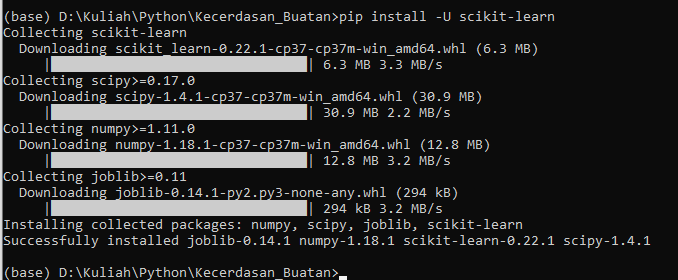
\includegraphics[width=4cm]{figures/1174035/chapter1/1_1.png}
		\centering
		\caption{Instalasi Scikit Learn}
	\end{figure}
	\item Setelah selesai instalasi, pilih salah satu example dari website Scikit (Contoh : \href{https://scikit-learn.org/stable/auto_examples/index.html})
	\begin{figure}[H]
		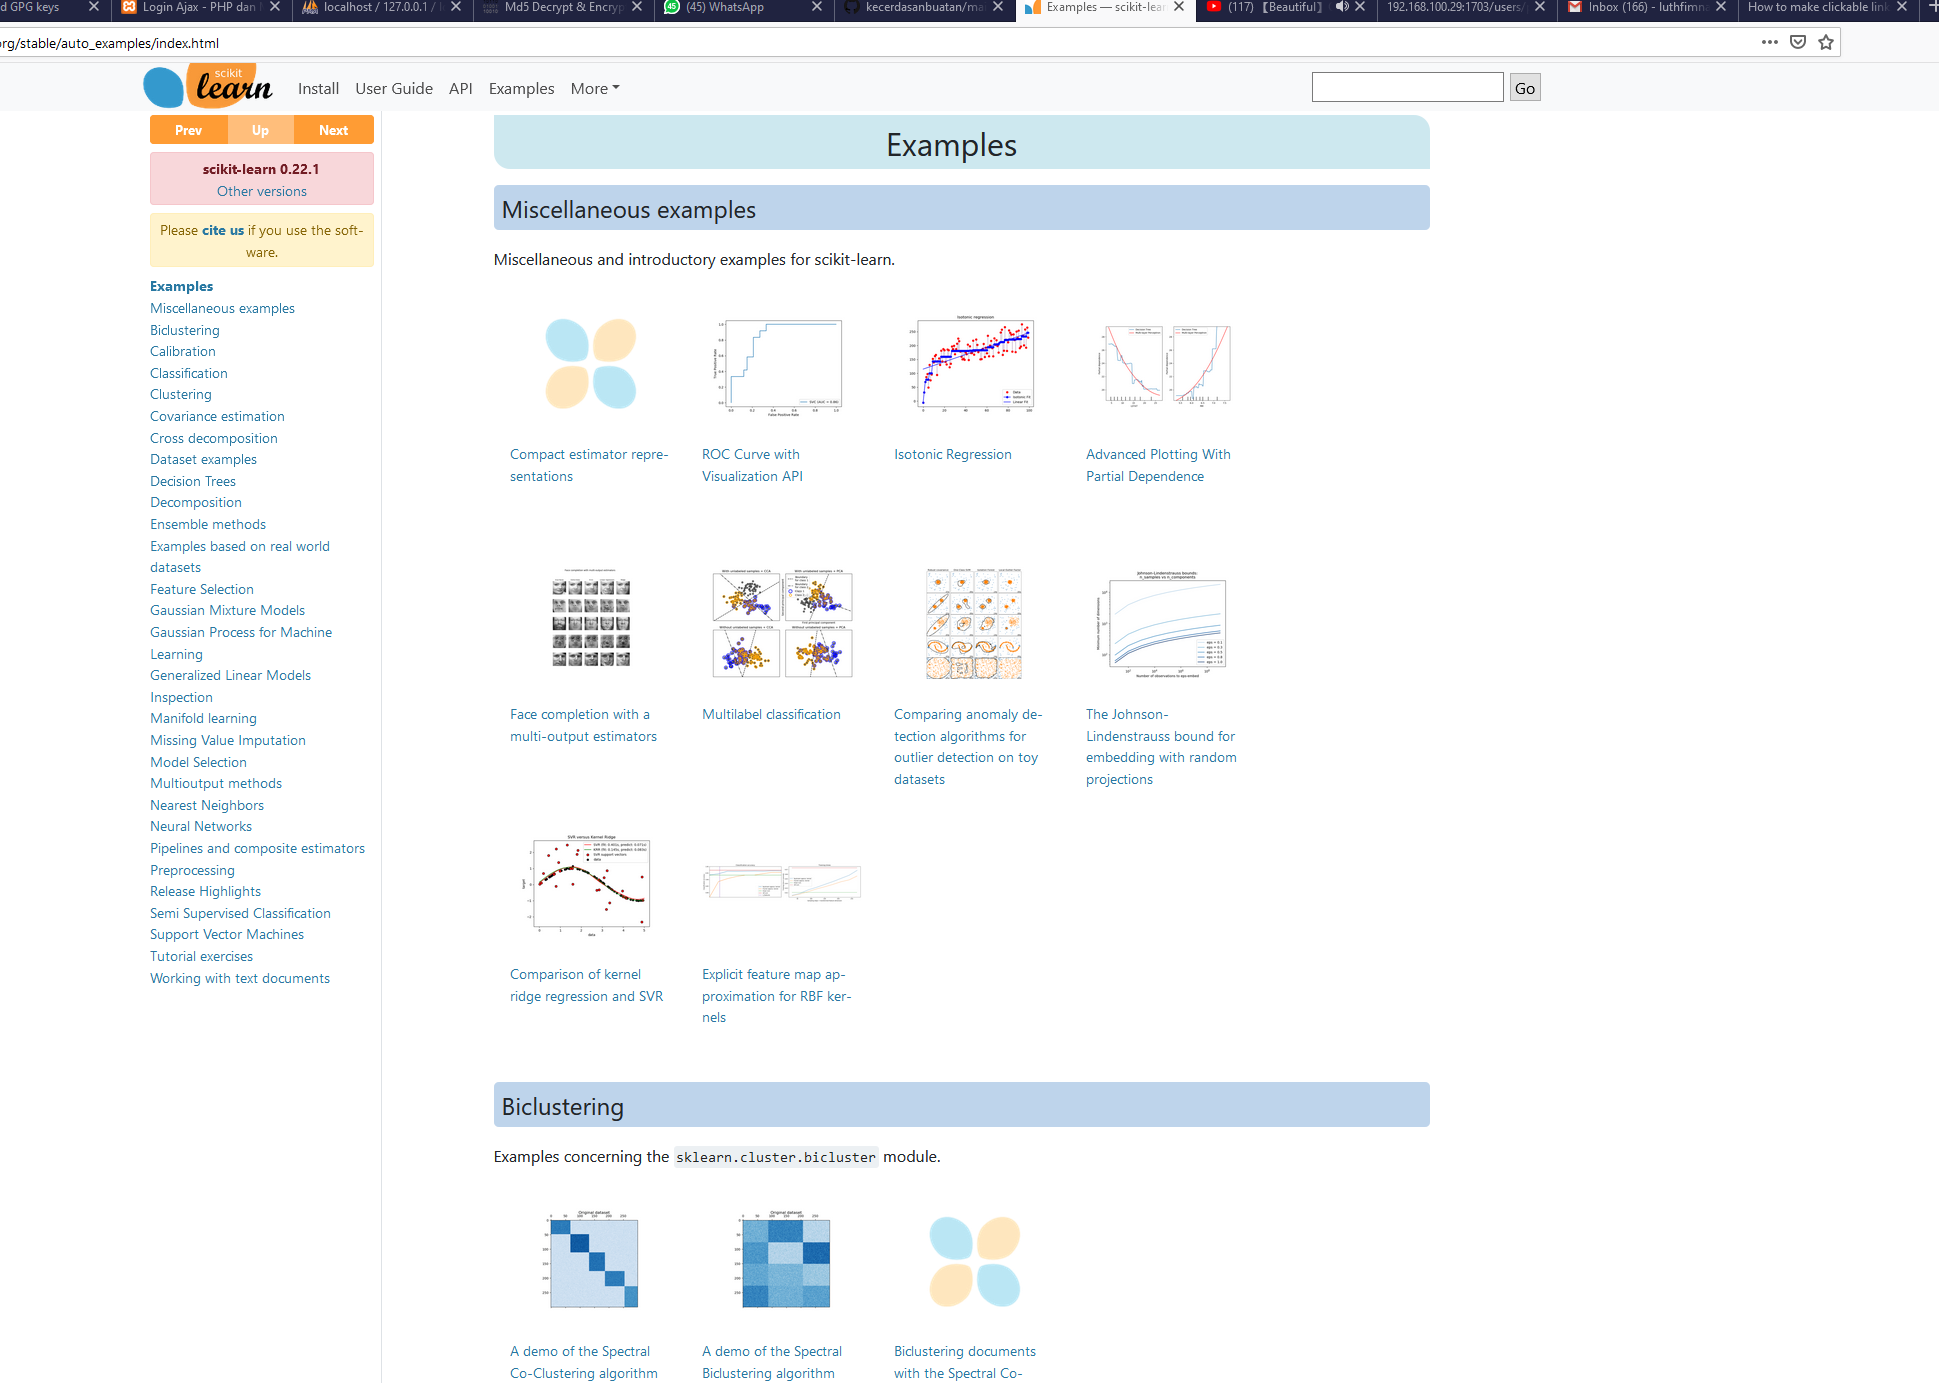
\includegraphics[width=4cm]{figures/1174035/chapter1/1_2.png}
		\centering
		\caption{Daftar Example}
	\end{figure}
	\item Lalu coba jalankan aplikasi tersebut, bisa dicek hasil dari Variable explorernya
	\begin{figure}[H]
		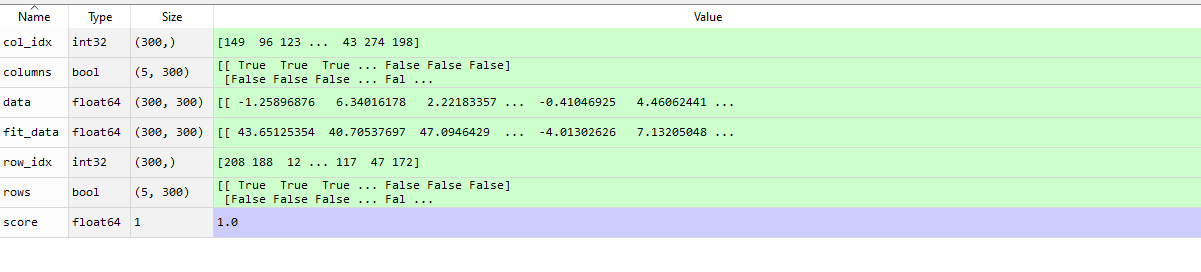
\includegraphics[width=4cm]{figures/1174035/chapter1/1_3.png}
		\centering
		\caption{Variable Explorer}
	\end{figure}
	\item Sample kode \hfill \break \lstinputlisting[firstline=1]{src/1174035/chapter1/sample1.py}
\end{enumerate}

\subsection{Mencoba Loading and example dataset}
\begin{itemize}
	\item Percobaan 1 (Memuat data iris dan digits dari datasets) \hfill \break \lstinputlisting[firstline=8, lastline=10]{src/1174035/chapter1/sample2.py}
	\begin{figure}[H]
		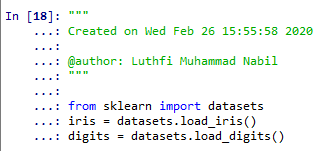
\includegraphics[width=4cm]{figures/1174035/chapter1/2_1_hasil.png}
		\centering
		\caption{Hasil Percobaan 1}
	\end{figure}
	\item Percobaan 2 (Menampilkan data dari digits) \hfill \break \lstinputlisting[firstline=12, lastline=12]{src/1174035/chapter1/sample2.py}
	\begin{figure}[H]
		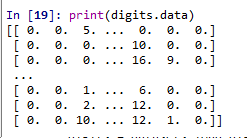
\includegraphics[width=4cm]{figures/1174035/chapter1/2_2_hasil.png}
		\centering
		\caption{Hasil Percobaan 2}
	\end{figure}
	\item Percobaan 3 (Menampilkan digits.target) \hfill \break \lstinputlisting[firstline=14, lastline=14]{src/1174035/chapter1/sample2.py}
	\begin{figure}[H]
		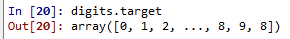
\includegraphics[width=4cm]{figures/1174035/chapter1/2_3_hasil.png}
		\centering
		\caption{Hasil Percobaan 3}
	\end{figure}
	\item Percobaan 4 (Menampilkan data 2 dimensi) \hfill \break \lstinputlisting[firstline=16, lastline=16]{src/1174035/chapter1/sample2.py}
	\begin{figure}[H]
		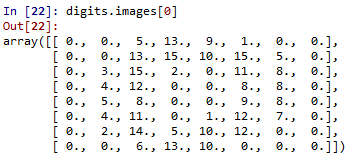
\includegraphics[width=4cm]{figures/1174035/chapter1/2_4_hasil.png}
		\centering
		\caption{Hasil Percobaan 4}
	\end{figure}
	\item Full sample \hfill \break \lstinputlisting[firstline=1]{src/1174035/chapter1/sample2.py}
	\begin{figure}[H]
		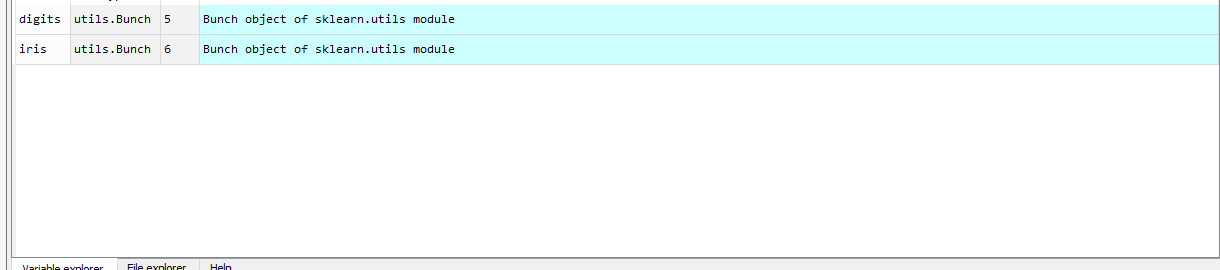
\includegraphics[width=4cm]{figures/1174035/chapter1/2_var.png}
		\centering
		\caption{Hasil pada variable explorer}
	\end{figure}
\end{itemize}
